\chapter{Implementasi dan Pengujian}
\label{chap:implementasi dan pengujian}

\section{Lingkungan Implementasi}
\label{sec:lingkungan implementasi}

Pada subab ini akan dipaparkan perangkat keras dan perangkat lunak yang digunakan dalam membangun sistem rekomendasi program studi Universitas Katolik Parahyangan.

\subsection{Lingkungan Perangkat Keras}
\label{sec:perangkat keras}

\begin{enumerate}
    \item Processor : Intel Core i5-7200
    
    \item Memory : 12 GB
    
    \item Harddisk : 1 T
    
    \item VGA : NVIDIA GeForce 940MX
\end{enumerate}

\section{Lingkungan Perangkat Lunak}
\label{sec:perangkat lunak}

\begin{enumerate}
    \item Web Server : Apache 2.4.41
    
    \item Tools : XAMPP 3.2.4 dan Visual Studio Code 1.44
    
    \item Bahasa Pemrograman : PHP 7.4.1
    
    \item Database management system : MySQL
    
    \item Operating System : Windows 10
\end{enumerate}

\section{Implementasi Tabel Basis Data}
\label{sec:implementasi tabel basis data}

Dibawah ini merupakan implementasi tabel basis data yang digunakan pada sistem rekomendasi program studi Universitas Katolik Parahyangan. 

\lstset{numbers=left}

\begin{enumerate}
    \item Tabel Jurusan SMA\\
    Tabel jurusan SMA digunakan untuk menyimpan seluruh data jurusan SMA yang digunakan pada sistem rekomendasi.
    
\begin{lstlisting}[language=SQL, caption=Implementasi tabel jurusan SMA]
CREATE TABLE `jurusan_sma` ( 
    `id_jurusan` int(10) UNSIGNED NOT NULL,
    `nama_jurusan` varchar(25) COLLATE utf8mb4_unicode_ci NOT NULL
) ENGINE=InnoDB DEFAULT CHARSET=utf8mb4 COLLATE=utf8mb4_unicode_ci;
\end{lstlisting}
    
    \item Tabel Fakultas\\
    Tabel fakultas digunakan untuk menyimpan seluruh fakultas yang ada di Universitas Katolik Parahyangan.
    
\begin{lstlisting}[language=SQL, caption=Implementasi tabel ]
CREATE TABLE `fakultas` (
    `id_fakultas` int(10) UNSIGNED NOT NULL,
    `nama_fakultas` varchar(50) COLLATE utf8mb4_unicode_ci NOT NULL
) ENGINE=InnoDB DEFAULT CHARSET=utf8mb4 COLLATE=utf8mb4_unicode_ci;    
\end{lstlisting}

    \item Program Studi\\
    Tabel program studi digunakan untuk menyimpan seluruh program studi yang ada di Universitas Katolik Parahyangan.
    
\begin{lstlisting}[language=SQL, caption=Implementasi tabel ]
CREATE TABLE `program_studi` (
    `id_program_studi` int(10) UNSIGNED NOT NULL,
    `nama_program_studi` varchar(50) COLLATE utf8mb4_unicode_ci NOT NULL,
    `id_fakultas` int(10) UNSIGNED NOT NULL,
    `id_jurusan` int(10) UNSIGNED NOT NULL
) ENGINE=InnoDB DEFAULT CHARSET=utf8mb4 COLLATE=utf8mb4_unicode_ci;
\end{lstlisting}
    
    \item Mahasiswa\\
    Tabel mahasiswa digunakan untuk menyimpan nilai seluruh mahasiswa yang sudah lulus dari Universitas Katolik Parahyangan.
    
\begin{lstlisting}[language=SQL, caption=Implementasi tabel ]
CREATE TABLE `mahasiswa` (
    `id_mahasiswa` int(10) UNSIGNED NOT NULL,
    `NPM` varchar(10) COLLATE utf8mb4_unicode_ci NOT NULL,
    `IPK` double(3,2) NOT NULL,
    `id_jurusan` int(10) UNSIGNED NOT NULL,
    `id_program_studi` int(10) UNSIGNED NOT NULL
) ENGINE=InnoDB DEFAULT CHARSET=utf8mb4 COLLATE=utf8mb4_unicode_ci;    
\end{lstlisting}
    
    \item Mata Pelajaran\\
    Tabel mata pelajaran digunakan untuk menyimpan mata pelajaran yang digunakan pada PMDK di Universitas Katolik Parahyangan.
    
\begin{lstlisting}[language=SQL, caption=Implementasi tabel ]
CREATE TABLE `mata_pelajaran` (
    `id_mata_pelajaran` int(10) UNSIGNED NOT NULL,
    `nama_mata_pelajaran` varchar(20) COLLATE utf8mb4_unicode_ci NOT NULL
) ENGINE=InnoDB DEFAULT CHARSET=utf8mb4 COLLATE=utf8mb4_unicode_ci;
\end{lstlisting}
    
    \item Nilai\\
    Tabel nilai digunakan untuk menyimpan nilai mahasiswa pada kelas X dan XI untuk semester 1 dan 2 pada saat SMA.
    
\begin{lstlisting}[language=SQL, caption=Implementasi tabel ]
CREATE TABLE `nilai` (
    `id_nilai` int(10) UNSIGNED NOT NULL,
    `id_mata_pelajaran` int(10) UNSIGNED NOT NULL,
    `id_mahasiswa` int(10) UNSIGNED NOT NULL,
    `101` double(5,2) NOT NULL,
    `102` double(5,2) NOT NULL,
    `111` double(5,2) NOT NULL,
    `112` double(5,2) NOT NULL,
    `AVG` double(5,2) NOT NULL
) ENGINE=InnoDB DEFAULT CHARSET=utf8mb4 COLLATE=utf8mb4_unicode_ci;
\end{lstlisting}
    
\end{enumerate}

\section{Impelemtasi Antar Muka}
\label{sec:implementasi antar muka}

Pada subab ini akan ditampilkan antar muka yang digunakan pada sistem rekomendasi program studi Universitas Katolik Parahyangan.

\begin{enumerate}
    \item Halaman index saat siswa/i mengakses sistem
    
    \begin{figure}[H]
        \centering
        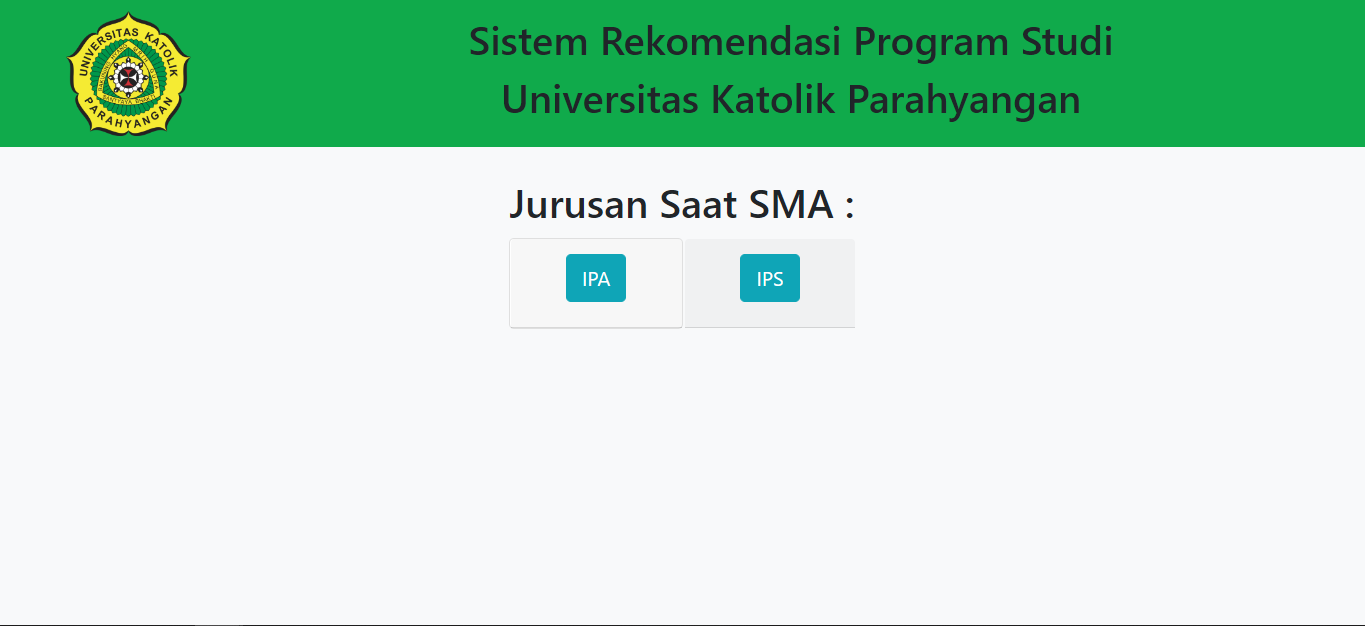
\includegraphics[width = 12cm, height =8 cm]{Gambar/gambar51.png}
        \caption{Halaman Index Sistem}
        \label{fig:gambar51}
    \end{figure}
    
    \item Halaman pengisisian nilai siswa/i IPA
    
    \begin{figure}[H]
        \centering
        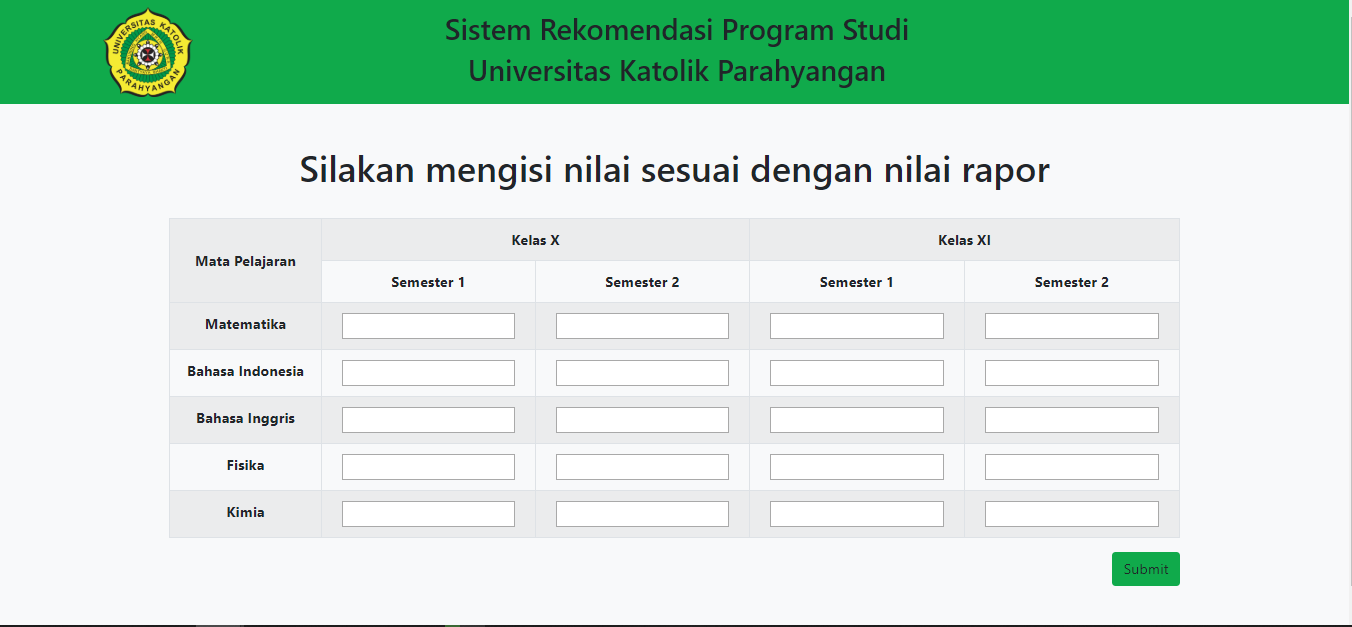
\includegraphics[width = 12cm, height =8 cm]{Gambar/gambar52.png}
        \caption{Halaman Index Pengisian Nilai IPA}
        \label{fig:gambar52}
    \end{figure}
    
    \item Halaman pengisisian nilai siswa/i IPS
    
    \begin{figure}[H]
        \centering
        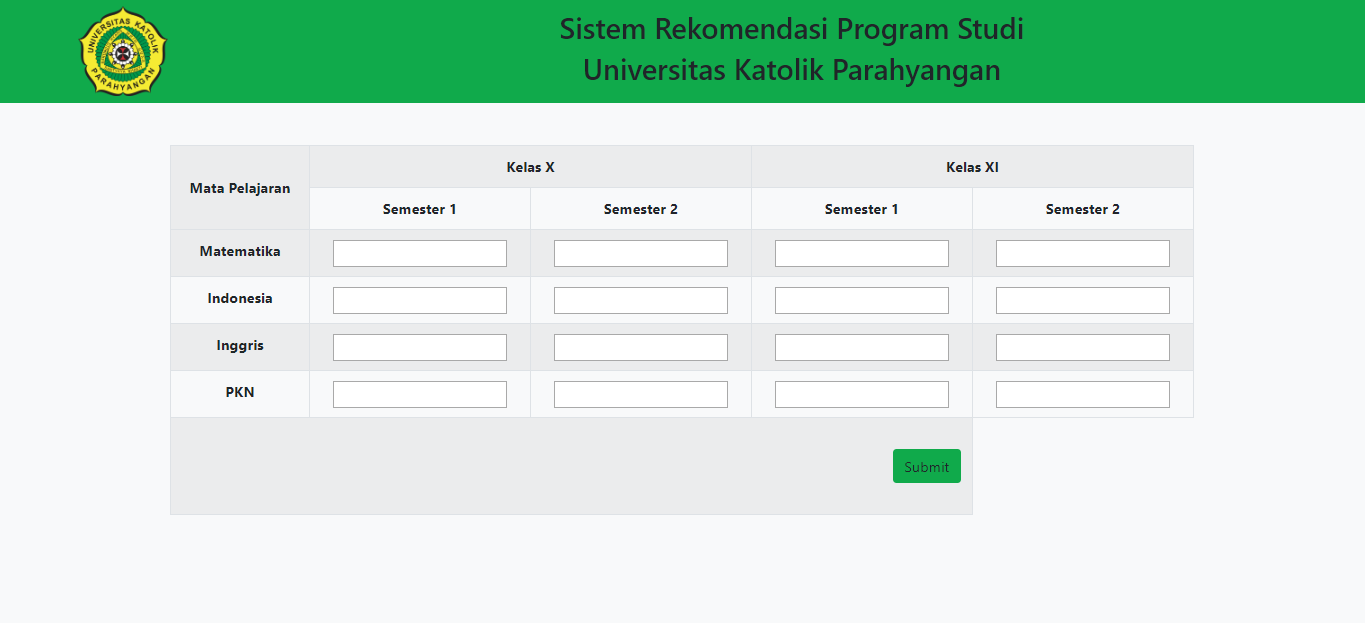
\includegraphics[width = 12cm, height =8 cm]{Gambar/gambar53.png}
        \caption{Halaman Index Pengisian Nilai IPS}
        \label{fig:gambar53}
    \end{figure}
    
    \item Halaman hasil rekomendasi
    \begin{figure}[H]
        \centering
        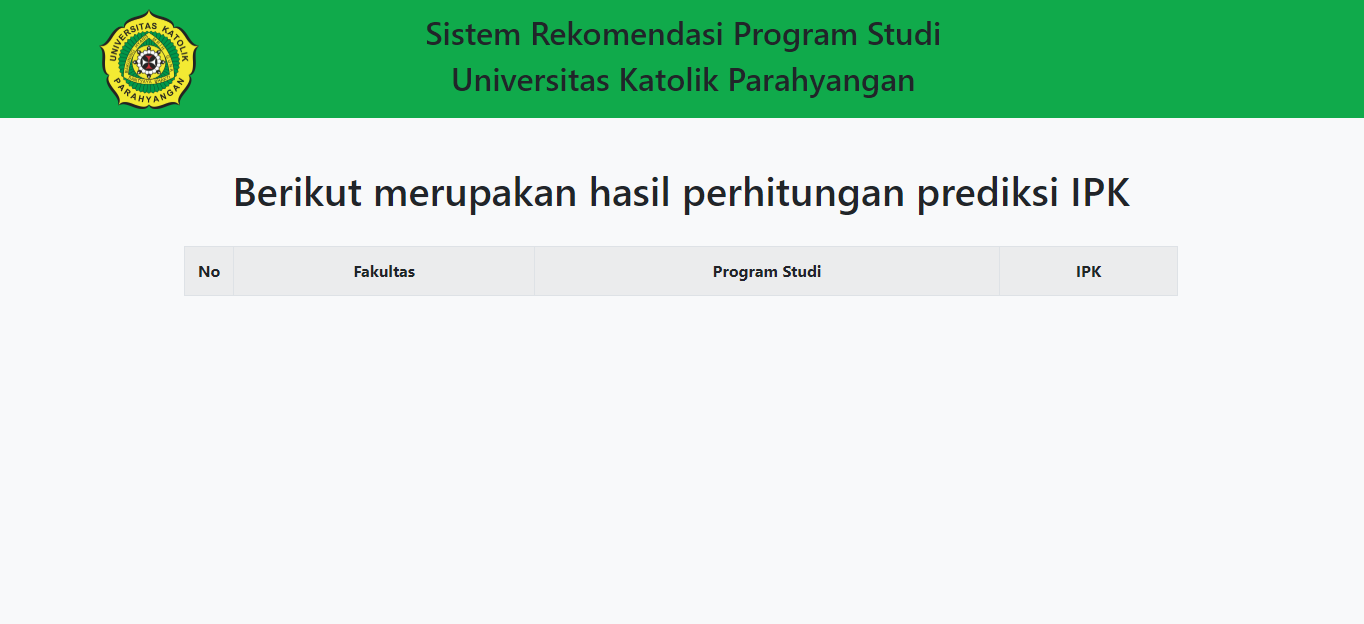
\includegraphics[width = 12cm, height =8 cm]{Gambar/gambar54.png}
        \caption{Halaman Hasil Rekomendasi}
        \label{fig:gambar54}
    \end{figure}
\end{enumerate}

\section{Pengujian Fungsional}
\label{sec:pengujian fungsional}

Pengujian ini dilakukan untuk menguji fitur-fitur yang ada pada sistem rekomendasi program studi Universitas Katolik Parahyangan agar dapat berjalan dengan baik.

\subsection{Pengujian Fungsional Pemilihan Jurusan SMA}
\label{subsec:pengujian fungsional pemilihan jurusan}

Pengujian ini dilakukan pada fitur pemilihan jurusan saat SMA oleh siswa/i yang menjadi target sistem.

\begin{table}[H]
    \centering
    \begin{tabular}{|c|p{3.5cm}|p{3.5cm}|p{3.5cm}|p{1.5cm}|}
        \hline
        No & Langkah Pengujian & Hasil yang diharapkan & Hasil Pengujian & Status \\
        \hline
        1 & Memilih juruusan saat SMA & Sistem mengarahkan kepada form sesuai jurusan SMA & Sistem mengarahkan kepada form sesuai jurusan SMA & Sesuai\\
        \hline
    \end{tabular}
    \caption{Tabel Pengujian Fungsional Pemilihan SMA}
    \label{tab:tabel pengujian fungsional pemilihan SMA}
\end{table}

\subsection{Pengujian Fungsional Pengisian Nilai}
\label{subsec:pengujian fungsional pengisian nilai}

Pengujian ini dilakukan pada fitur pengisian nilai mata pelajaran sesuai dengan jurusan saat SMA pada kelas X dan XI. 

\begin{table}[H]
    \centering
    \begin{tabular}{|c|p{3.5cm}|p{3.5cm}|p{3.5cm}|p{1.5cm}|}
        \hline
        No & Langkah Pengujian & Hasil yang diharapkan & Hasil Pengujian & Status \\
        \hline
        1 & Mengisi nilai sesuai nilai rapor & Memeriksa valid tidaknya data yang dimasukkan dan memeriksa \textit{range} nilai & Memeriksa valid tidaknya data yang dimasukkan dan memeriksa \textit{range} nilai & Sesuai \\
        \hline
        2 & Klik tombol \textit{submit} & Mengerahkan kepada halaman hasil rekomendasi & Mengerahkan kepada halaman hasil rekomendasi & Sesuai \\
        \hline
        3 & Mengisi nilai yang tidak valid & Memberikan pesan data tidak valid & Memberikan pesan data tidak valid & Sesuai\\
        \hline
    \end{tabular}
    \caption{Tabel Pengujian Fungsional Pengisian Nilai}
    \label{tab:tabel pengujian fungsional pengisian nilai}
\end{table}


\section{Pengujian Eksperimental}
\label{sec:pengujian eksperimental}

Pada subab ini, akan dilakukkan pengujian sistem rekomendasi program studi Universitas Katolik Parahyangan. Pengujian dilakukan menggunakan \textit{Mean Absolute Error} (MAE), \textit{Root Mean Square Error} (RMSE), dan eksekusi waktu program. Data yang digunakan pada pengujian adalah seluruh data mahasiswa yang dibagi menjadi dua yaitu \textit{train set} sebesar 70\% dan \textit{test set} sebesar 30\%. Pengujian dilakukkan dengan dua metode, yaitu : 

\subsection{Metode Dasar}
\label{subsec: metode dasar}

Metode dasar ini dilakukkan dengan cara menguji secara langsung \textit{test set} kedalam sistem dengan menggunakan \textit{train set}. Berikut merupakan hasil pengujian dengan metode dasar :

\begin{enumerate}
    \item IPA
        \begingroup
        \renewcommand\arraystretch{1.5}
            \begin{longtable}[H]{|c|c|c|c|}
                \hline
                No & MAE & RMSE & Time\\
                \hline
                1 & 0.2754545455 & 0.3495110995 & 0.002562046051\\
                \hline
                2 & 0.2718614719 & 0.330867939 & 0.002246141434\\
                \hline
                3 & 0.2943290043 & 0.3680562022 & 0.00180888176\\
                \hline 
                4 & 0.2781659389 & 0.3533915527 & 0.002074956894\\
                \hline 
                5 & 0.2694805195 & 0.3351777974 & 0.00253200531\\
                \hline 
                6 & 0.2818181818 & 0.3456570379 & 0.00125002861\\
                \hline 
                7 & 0.2858008658 & 0.363914504 & 0.001752138138\\
                \hline 
                8 & 0.2703896104 & 0.3409561295 & 0.003805160522\\
                \hline 
                9 & 0.2937662338 & 0.3675235953 & 0.00479888916\\
                \hline 
                10 & 0.2926839827 & 0.3660287643 & 0.002127885818\\
                \hline
                
                \caption{Hasil Pengujian Jurusan IPA dengan Metode Dasar}
                \label{tab:pengujian ipa dasar}
            \end{longtable}
        \endgroup
        
    \item IPS
        \begingroup
        \renewcommand\arraystretch{1.5}
            \begin{longtable}[H]{|c|c|c|c|}
                \hline
                No & MAE & RMSE & Time\\
                \hline
                1 & 0.2944 & 0.3655757104 & 0.003097057343\\
                \hline
                2 & 0.29092 & 0.3719166573 & 0.002082824707\\
                \hline
                3 & 0.28344 & 0.3553927405 & 0.00294303894\\
                \hline
                4 & 0.286064257 & 0.3595384145 & 0.001393079758\\
                \hline
                5 & 0.3212851406 & 0.3974486908 & 0.001703023911\\
                \hline
                6 & 0.29276 & 0.3556430795 & 0.002462148666\\
                \hline
                7 & 0.28544 & 0.3532149487 & 0.001994848251\\
                \hline
                8 & 0.2704 & 0.3468486702 & 0.001998186111\\
                \hline
                9 & 0.27304 & 0.3416021077 & 0.00242805481\\
                \hline
                10 & 0.28952 & 0.3625961941 & 0.001628875732\\
                \hline
                
                \caption{Hasil Pengujian Jurusan IPS dengan Metode Dasar}
                \label{tab:pengujian ips dasar}
            \end{longtable}
        \endgroup
        
\end{enumerate}

\subsection{Metode KMeans}
\label{subsec: metode kmeans}

Metode KMeans dilakukkan dengan membuat kelompok dari \textit{train set} dan menentukan \textit{test set} masuk kedalam kelompok mana, untuk mengurangi perhitungan kemiripan atau similaritas dengan pengguna yang memiliki kemiripan kecil atau tidak memiliki kemiripan sama sekali. Pada pengujian ini dilakukan dengan nilai maksimum 10, 20, 30, dan 40 dengan pengulangan dalam pembentukan kelompok sebanyak 30 kali. Berikut merupakan hasil pengujian yang dilakukan dengan menggunkan k-means dengan mimilih nilai minimum dari k = 2 sampai k = n (n = 10, 20, 30, dan 40) :

%Pada pengujian ini dilakukkan dengan nilai k 2 sampai 10 dan dilakukkan pengulangan dalam pembentuk kelompok sebanyak 30 kali. Gambar \ref{fig:pengujian ipa kmeans} dan gambar \ref{fig:pengujian ips kmeans} merupakan hasil perhitungan untuk \textit{Mean Absolute Error} (MAE), \textit{Root Mean Square Error} (RMSE), dan eksekusi waktu program.

\begin{enumerate}
    \item IPA
        \begin{enumerate}
            \item k = 10 \\
                \begingroup
                \renewcommand\arraystretch{1.5}
                    \begin{longtable}[H]{|c|c|c|c|c|c|c|}
                        \hline
                        No & k & MAE & k & RMSE & k & Time \\
                        \hline
                        1 & 10 & 0.227403435  & 10 & 0.299831433 & 9 & 39.32930207\\
                        \hline
                        2 & 10 & 0.2319802782  & 10 & 0.3163842676 & 8 & 44.21230698\\
                        \hline
                        3 & 9 & 0.2378234118 & 9 & 0.3031256224 & 8 & 97.19740295\\
                        \hline
                        4 & 10 & 0.2258213385 & 10 & 0.3049147694 & 10 & 84.33423114\\
                        \hline
                        5 & 10 & 0.2424204718 & 10 & 0.3144518957 & 6 & 98.56704521\\
                        \hline
                        6 & 10 & 0.2313912291 & 10 & 0.3061390768 & 7 & 92.61572003\\
                        \hline
                        7 & 10 & 0.2218367518 & 8 & 0.2863855107 & 7 & 91.99784708\\
                        \hline
                        8 & 10 & 0.2385816174 & 10 & 0.317593614 & 9 & 90.1020081\\
                        \hline
                        9 & 9 & 0.235875589 & 9 & 0.3079230922 & 10 & 43.22178102\\
                        \hline
                        10 & 10 & 0.2311139896 & 7 & 0.3090021998 & 10 & 42.38479996\\
                        \hline
                        
                        \caption{Hasil Pengujian KMeans Jurusan IPA dengan nilai k 10}
                        \label{tab:ipa k = 10}
                    \end{longtable}
                \endgroup
            
            Berdasarkan tabel \ref{tab:ipa k = 10} MAE memiliki nilai rata-rata 0.2324248112, RMSE memiliki nilai rata-rata 0.3065751482, dan \textit{Time} memiliki nilai rata-rata 72.39624445. Nilai k yang sering muncul pada pengujian ini untuk nilai minimum MAE, RMSE, dan \textit{Time} adalah 10.
            
            \item k = 20 \\
                \begingroup
                \renewcommand\arraystretch{1.5}
                    \begin{longtable}[H]{|c|c|c|c|c|c|c|}
                        \hline
                        No & k & MAE & k & RMSE & k & Time \\
                        \hline
                        1 & 20 & 0.2368744669 & 20 & 0.3267037296 & 9 & 37.72296405\\
                        \hline
                        2 & 20 & 0.2296986147 & 20 & 0.3141882874 & 11 & 43.61491799\\
                        \hline
                        3 & 19 & 0.2120384835 & 18 & 0.2788791667 & 10 & 42.64620209\\
                        \hline
                        4 & 20 & 0.2241357999 & 16 & 0.3006233447 & 16 & 80.17571688\\
                        \hline
                        5 & 20 & 0.2043304288 & 20 & 0.2822296445 & 15 & 85.85764313\\
                        \hline
                        6 & 20 & 0.2306250152 & 20 & 0.3119114291 & 14 & 83.94621801\\
                        \hline
                        7 & 20 & 0.2296141379 & 12 & 0.2954344085 & 15 & 40.83648014\\
                        \hline
                        8 & 17 & 0.2243950223 & 15 & 0.2893674473 & 10 & 39.863837\\
                        \hline
                        9 & 20 & 0.2216946395 & 20 & 0.2922878602 & 7 & 40.8350091\\
                        \hline
                        10 & 19 & 0.240638961 & 17 & 0.3306430269 & 14 & 46.11702394\\
                        \hline
                        
                        \caption{Hasil Pengujian KMeans Jurusan IPA dengan nilai k 20}
                        \label{tab:ipa k = 20}
                    \end{longtable}
                \endgroup
                
                Berdasarkan tabel \ref{tab:ipa k = 20} MAE memiliki nilai rata-rata 0.225404557, RMSE memiliki nilai rata-rata 0.3022268345, dan \textit{Time} memiliki nilai rata-rata 54.16160123. Nilai k yang sering muncul pada pengujian ini untuk nilai minimum MAE dan RMSE adalah 20, sedangkan untuk \textit{Time} adalah 10.
                
            \item k = 30 \\
                \begingroup
                \renewcommand\arraystretch{1.5}
                    \begin{longtable}[H]{|c|c|c|c|c|c|c|}
                        \hline
                        No & k & MAE & k & RMSE & k & Time \\
                        \hline
                        1 & 28 & 0.2273780792 & 29 & 0.3056258724 & 21 & 49.22187304\\
                        \hline
                        2 & 29 & 0.2306341231 & 28 & 0.3163753408 & 14 & 38.71597004\\
                        \hline
                        3 & 28 & 0.2316359452 & 24 & 0.3212528501 & 11 & 37.75750303\\
                        \hline
                        4 & 29 & 0.2177379451 & 30 & 0.2987796808 & 10 & 40.64227509\\
                        \hline
                        5 & 26 & 0.2220062121 & 26 & 0.3098835924 & 16 & 78.95163608\\
                        \hline
                        6 & 30 & 0.2155065123 & 30 & 0.2841334884 & 15 & 78.09852815\\
                        \hline
                        7 & 30 & 0.2048133794 & 23 & 0.2865483893 & 21 & 42.30235791\\
                        \hline
                        8 & 28 & 0.2421590232 & 22 & 0.3291719967 & 11 & 36.66157508\\
                        \hline
                        9 & 29 & 0.2013756381 & 25 & 0.2824283764 & 13 & 36.40050817\\
                        \hline
                        10 & 30 & 0.224918007 & 28 & 0.3073142264 & 18 & 38.90666604\\
                        \hline
                        
                        \caption{Hasil Pengujian KMeans Jurusan IPA dengan nilai k 30}
                        \label{tab:ipa k = 30}
                    \end{longtable}
                \endgroup
                
                Berdasarkan tabel \ref{tab:ipa k = 30} MAE memiliki nilai rata-rata 0.2218164865, RMSE memiliki nilai rata-rata 0.3041513814, dan \textit{Time} memiliki nilai rata-rata 47.76588926. Nilai k yang sering muncul pada pengujian ini untuk nilai minimum MAE dan RMSE adalah 28, sedangkan \textit{Time} adalah 21.
                
            \item k = 40 \\
                \begingroup
                \renewcommand\arraystretch{1.5}
                    \begin{longtable}[H]{|c|c|c|c|c|c|c|}
                        \hline
                        No & k & MAE & k & RMSE & k & Time \\
                        \hline
                        1 & 40 & 0.2261115139 & 39 & 0.3148696499 & 7 & 53.68976092\\
                        \hline
                        2 & 40 & 0.210807028 & 40 & 0.2941391462 & 39 & 40.15380907\\
                        \hline
                        3 & 38 & 0.2316407044 & 38 & 0.311780573 & 22 & 47.243294\\
                        \hline
                        4 & 40 & 0.1895366044 & 39 & 0.2741478646 & 15 & 36.78319001\\
                        \hline
                        5 & 40 & 0.1833267575 & 32 & 0.2594329792 & 24 & 78.36255598\\
                        \hline
                        6 & 40 & 0.2097968665 & 34 & 0.2893972683 & 27 & 46.24171209\\
                        \hline
                        7 & 38 & 0.2021653817 & 38 & 0.2806167454 & 12 & 35.07260013\\
                        \hline
                        8 & 40 & 0.2231380327 & 28 & 0.3055987843 & 13 & 84.48507595\\
                        \hline
                        9 & 40 & 0.2081731563 & 26 & 0.2899252581 & 19 & 40.49293399\\
                        \hline
                        10 & 37 & 0.2129012891 & 37 & 0.302792602 & 19 & 38.59012914\\
                        \hline
                        
                        \caption{Hasil Pengujian KMeans Jurusan IPA dengan nilai k 40}
                        \label{tab:ipa k = 40}
                    \end{longtable}
                \endgroup
                
                Berdasarkan tabel \ref{tab:ipa k = 40} MAE memiliki nilai rata-rata 0.2097597334, RMSE memiliki nilai rata-rata 0.2922700871, dan \textit{Time} memiliki nilai rata-rata 50.11150613. Nilai k yang sering muncul pada pengujian ini untuk nilai minimum MAE adalah 40, RMSE adalah 39, dan \textit{Time} adalah 19.
                
        \end{enumerate}
        
        
        
    \item IPS
        \begin{enumerate}
            \item k = 10 \\
                \begingroup
                \renewcommand\arraystretch{1.5}
                    \begin{longtable}[H]{|c|c|c|c|c|c|c|}
                        \hline
                        No & k & MAE & k & RMSE & k & Time \\
                        \hline
                        1 & 10 & 0.2471143679 & 10 & 0.3158455625 & 10 & 54.29916787\\
                        \hline
                        2 & 10 & 0.2620947798 & 7 & 0.3363475028 & 10 & 52.25956702\\
                        \hline
                        3 & 10 & 0.244470971 & 9 & 0.3165210982 & 10 & 49.05109715\\
                        \hline
                        4 & 10 & 0.2518617969 & 10 & 0.3158170943 & 9 & 46.56690907\\
                        \hline
                        5 & 10 & 0.2553253166 & 10 & 0.3150100854 & 6 & 48.13360286\\
                        \hline
                        6 & 10 & 0.2849076998 & 10 & 0.3541113867 & 10 & 109.8035731\\
                        \hline
                        7 & 10 & 0.2757233651 & 10 & 0.3471834944 & 5 & 133.003581\\ 
                        \hline
                        8 & 10 & 0.2850747681 & 9 & 0.3568411162 & 10 & 102.0692439\\
                        \hline
                        9 & 10 & 0.2529911624 & 10 & 0.3205667096 & 7 & 110.884131\\
                        \hline
                        10 & 9 & 0.258458903 & 8 & 0.3287219636 & 7 & 111.2748449\\
                        \hline
                        10 & 10 & 0.2618023131 & 10 & 0.3306966014 & 10 & 81.73457179\\
                        \hline
                        
                        \caption{Hasil Pengujian KMeans Jurusan IPS dengan nilai k 10}
                        \label{tab:ips k = 10}
                    \end{longtable}
                \endgroup
                
                Berdasarkan tabel \ref{tab:ips k = 10} MAE memiliki nilai rata-rata 0.2618023131, RMSE memiliki nilai rata-rata 0.3306966014, dan \textit{Time} memiliki nilai rata-rata 81.73457179. Nilai k yang sering muncul pada pengujian ini untuk nilai minimum MAE, RMSE, \textit{Time} adalah 10.
                
                
            \item k = 20 \\
                \begingroup
                \renewcommand\arraystretch{1.5}
                    \begin{longtable}[H]{|c|c|c|c|c|c|c|}
                        \hline
                        No & k & MAE & k & RMSE & k & Time \\
                        \hline
                        1 & 20 & 0.2479751448 & 14 & 0.320530291 & 15 & 131.4302571\\
                        \hline
                        2 & 20 & 0.2699991293 & 20 & 0.3439232209 & 18 & 58.75904799\\
                        \hline
                        3 & 20 & 0.2526969538 & 20 & 0.3247280295 & 18 & 58.01726198\\
                        \hline
                        4 & 20 & 0.2449429082 & 20 & 0.3172577351 & 15 & 108.4736061\\
                        \hline
                        5 & 20 & 0.2508308575 & 18 & 0.3329961122 & 11 & 112.740905\\
                        \hline
                        6 & 19 & 0.245467054 & 16 & 0.327941758 & 20 & 52.00171995\\
                        \hline
                        7 & 20 & 0.2630213462 & 20 & 0.3362285177 & 19 & 47.86454606\\
                        \hline
                        8 & 20 & 0.2581428437 & 16 & 0.3259706399 & 6 & 44.44093394\\
                        \hline
                        9 & 19 & 0.2431999995 & 19 & 0.3203262814 & 6 & 51.23832917\\
                        \hline
                        10 & 20 & 0.2635233778 & 19 & 0.3371743255 & 7 & 58.85741878\\
                        \hline
                        
                        \caption{Hasil Pengujian KMeans Jurusan IPS dengan nilai k 20}
                        \label{tab:ips k = 20}
                    \end{longtable}
                \endgroup
                
                Berdasarkan tabel \ref{tab:ips k = 20} MAE memiliki nilai rata-rata 0.2539799615, RMSE memiliki nilai rata-rata 0.3287076911, dan \textit{Time} memiliki nilai rata-rata 72.38240261. Nilai k yang sering muncul pada pengujian ini untuk nilai minimum MAE dan RMSE adalah 20, sedangkan \textit{Time} adalah 15.
                
            \item k = 30 \\
                \begingroup
                \renewcommand\arraystretch{1.5} 
                    \begin{longtable}[H]{|c|c|c|c|c|c|c|}
                        \hline
                        No & k & MAE & k & RMSE & k & Time \\
                        \hline
                        1 & 28 & 0.2465264584 & 22 & 0.3219106761 & 9 & 112.462486\\
                        \hline
                        2 & 30 & 0.2354540964 & 30 & 0.303054355 & 28 & 48.99936104\\
                        \hline
                        3 & 30 & 0.2549761589 & 30 & 0.3345880728 & 23 & 47.77446008\\
                        \hline
                        4 & 30 & 0.2291845383 & 30 & 0.3143040765 & 22 & 50.10031199\\
                        \hline
                        5 & 27 & 0.2326224221 & 27 & 0.300938373 & 14 & 51.63516593\\
                        \hline
                        6 & 30 & 0.2506048091 & 26 & 0.3260176261 & 9 & 93.11268997\\
                        \hline
                        7 & 29 & 0.235422277 & 23 & 0.3065052835 & 29 & 48.41273594\\
                        \hline
                        8 & 29 & 0.2544741621 & 29 & 0.331396395 & 5 & 57.45985603\\
                        \hline
                        9 & 30 & 0.2402659051 & 29 & 0.3166005062 & 29 & 54.32228708\\
                        \hline
                        10 & 29 & 0.2219832516 & 29 & 0.294076226 & 29 & 53.01417494\\
                        \hline
                        
                        
                        \caption{Hasil Pengujian KMeans Jurusan IPS dengan nilai k 30}
                        \label{tab:ips k = 30}
                    \end{longtable}
                \endgroup
                
                Berdasarkan tabel \ref{tab:ips k = 30} MAE memiliki nilai rata-rata 0.2401514079, RMSE memiliki nilai rata-rata 0.2855315364, dan \textit{Time} memiliki nilai rata-rata 61.7293529. Nilai k yang sering muncul pada pengujian ini untuk nilai minimum MAE dan RMSE adalah 30, sedangkan \textit{Time} adalah 29.
                
            \item k = 40 \\
                \begingroup
                \renewcommand\arraystretch{1.5}
                    \begin{longtable}[H]{|c|c|c|c|c|c|c|}
                        \hline
                        No & k & MAE & k & RMSE & k & Time \\
                        \hline
                        
                        
                        \caption{Hasil Pengujian KMeans Jurusan IPS dengan nilai k 40}
                        \label{tab:ips k = 40}
                    \end{longtable}
                \endgroup
                
                Berdasarkan tabel \ref{tab:ips k = 40} MAE memiliki nilai rata-rata, RMSE memiliki nilai rata-rata, dan \textit{Time} memiliki nilai rata-rata . Nilai k yang sering muncul pada pengujian ini untuk nilai minimum MAE, RMSE, \textit{Time} adalah .
        \end{enumerate}
\end{enumerate}

%Dari hasil pengujian baik menggunakan metode \ref{subsec: metode dasar} dan metode \ref{subsec: metode kmeans} dengan jurusan IPA pada gambar \ref{fig:pengujian ipa kmeans} nilai MAE dan RMSE terkecil terdapat pada k = 10 dan eksekusi waktu program terdapat pada k = 9 dengan selisih 1.05433297 \textit{mic sec} dan jurusan IPS dengan nilai MAE, RMSE, dan eksekusi waktu program terdapat pada k = 10.

\subsection{Kesimpulan Hasil Pengujian}
\label{subsec:kesimpulan hasil pengujian}

\begin{enumerate}
    \item Metode Dasar 
        \begin{enumerate}
            \item IPA \\
                Berdasarkan tabel \ref{tab:pengujian ipa dasar} pengujian ipa dasar nilai MAE memiliki nilai rata-rata 0.2813750354, RMSE memiliki nilai rata-rata 0.3521084622, dan \textit{Time} memiliki nilai rata-rata 0.00249581337.
            
            \item IPS \\
                Berdasarkan tabel \ref{tab:pengujian ips dasar} pengujian ips dasar nilai MAE memiliki nilai rata-rata 0.2887269398, RMSE memiliki nilai rata-rata 0.3609777214, dan \textit{Time} memiliki nilai rata-rata 0.002173113823.
                
        \end{enumerate}
    
    \item Metode K-Means
        \begin{enumerate}
            \item IPA
                \begingroup
                    \renewcommand\arraystretch{1.5}
                    \begin{longtable}{|c|c|c|c|c|c|c|}
                        \hline
                        \multirow{2}{*}{K} & k & MAE & k & RMSE & k & Time \\
                        & dominan & & dominan & & dominan & \\
                        \hline
                        10 & 10 & 0.2324248112 & 10 & 0.3065751482 & 10 & 72.39624445\\
                        \hline
                        20 & 20 & 0.225404557 & 20 & 0.3022268345 & 10 & 54.16160123\\
                        \hline
                        30 & 28 & 0.2218164865 & 28 & 0.3041513814 & 21 & 47.76588926\\
                        \hline
                        40 & 40 & 0.2097597334 & 39 & 0.2922700871 & 19	 & 50.11150613\\
                        \hline
                        
                        \caption{Hasil Pengujian Jurusan IPA}
                        \label{tab:hasil pengujian ipa}
                    \end{longtable}
                \endgroup
                
                Berdasarkan hasil pengujian jurusan IPA dengan metode K-Means pada tabel \ref{tab:hasil pengujian ipa} yang menampilkan k dominan dan rata-rata untuk MAE, RMSE, dan \textit{Time}. Nilai rata-rata MAE terkecil adalah 0.2097597334 dengan k 40, rata-rata RMSE terkecil adalah 0.2922700871 dengan k 39, dan rata-rata \textit{Time} terkecil adalah 47.76588926 dengan k 21.
                
                
            \item IPS
                \begingroup
                    \renewcommand\arraystretch{1.5}
                    \begin{longtable}{|c|c|c|c|c|c|c|}
                        \hline
                        \multirow{2}{*}{K} & k & MAE & k & RMSE & k & Time \\
                        & dominan & & dominan & & dominan & \\
                        \hline
                        10 & 10 & 0.2618023131 & 10 & 0.3306966014 & 10 & 81.73457179\\
                        \hline
                        20 & 20 & 0.2539799615 & 20 & 0.3287076911 & 15 & 72.38240261\\
                        \hline
                        30 & 30 & 0.2401514079 & 30 & 0.2855315364 & 29 & 61.7293529\\
                        \hline
                        
                        \caption{Hasil Pengujian Jurusan IPS}
                        \label{tab:hasil pengujian ips}
                    \end{longtable}
                \endgroup
                
                Berdasarkan hasil pengujian jurusan IPS dengan metode K-Means pada tabel \ref{tab:hasil pengujian ips} yang menampilkan k dominan dan rata-rata untuk MAE, RMSE, dan \textit{Time}. Nilai rata-rata MAE terkecil adalah  dengan k , rata-rata RMSE terkecil adalah  dengan k , dan rata-rata \textit{Time} terkecil adalah  dengan k .
                
        \end{enumerate}
        
\end{enumerate}